\documentclass[11pt]{article}
\usepackage[T1]{fontenc}
\usepackage[margin=0.9in]{geometry}
\usepackage{amsmath,booktabs,float,graphicx}
\usepackage[hidelinks]{hyperref}
\usepackage{microtype}
\setlength{\emergencystretch}{1em}
\title{Does Image Disagreement Help Decide Which Breast Ultrasound Predictions to Defer?}
\author{Bahodir Nazarov, Zineb Gharib, Fatima Zazoul, and Luo Chuan}
\date{}
\begin{document}
\maketitle

\begin{abstract}
\textbf{Purpose.} We test whether disagreement between two breast ultrasound image scores helps rank patient-level errors after accounting for confidence in the average score.

\textbf{Methods.} We use 1,875 image records from 1,064 BUS-BRA patient groups, including 811 two-image groups. We compare confidence-only and confidence-plus-disagreement error rankers using patient-disjoint nested splits with logistic regression and histogram gradient boosting. Secondary analyses test frozen cutoffs, held-out scanners, and an alternate feature set generated from the public archive.

\textbf{Results.} Adding disagreement changed area under the generalized risk--coverage curve by $-0.011$ percentage points with logistic regression (paired patient-bootstrap 95\% interval $[-0.056,0.033]$) and by $-0.045$ points with gradient boosting ($[-0.131,0.038]$). With a confidence-only cutoff set to retain at least 90\% of separate calibration patients, the logistic model retained 90.6\% of test patients overall, including 83.4\% of malignant and 94.1\% of benign cases. The benign-minus-malignant coverage gap was 10.7 points (95\% interval $[6.1,15.5]$).

\textbf{Conclusion.} The incremental benefit of absolute score disagreement was uncertain in this cohort. The frozen cutoff retained fewer malignant cases proportionally, supporting diagnosis-specific reporting alongside overall coverage.
\end{abstract}

\section{Introduction}
A classifier that can defer a prediction trades off the number of cases it classifies against the errors it leaves among those cases \cite{geifman}. When several images belong to a patient, the spread between their model scores offers a candidate signal for deferral. A useful test is whether the spread improves error ranking after accounting for confidence in the patient-level decision. A second concern is whether an acceptable overall coverage rate can coexist with unequal coverage by diagnosis.

We study these questions using prepared radiomic measurements from BUS-BRA \cite{busbra}. We hold patient-level decisions fixed within each comparison, so differences in risk reflect which cases are retained. We measure errors retained across the coverage range and estimate diagnosis-specific coverage when the cutoff is set before seeing the test patients.

\section{Related work}
Wei et al.\ combined two ultrasound views for classification \cite{wei}. We use two image scores to rank the errors of a fixed patient decision. Geifman and El-Yaniv formalized the selective-classification trade-off between risk and coverage \cite{geifman}. Traub et al.\ proposed AUGRC to summarize generalized risk over the coverage range \cite{traub}. Jones et al.\ showed that selective classification can affect groups unevenly \cite{jones}. We examine retention by pathology label to characterize the composition of a retrospective review queue. Kinalioglu evaluated conformal reliability on held-out BUS-BRA scanners \cite{kinalioglu}. Our scanner analysis asks whether disagreement adds value for ranking patient-level errors and how coverage changes with a cutoff fitted on source-device patients.

\section{Materials and methods}
\subsection{Data and training boundaries}
BUS-BRA contains 1,875 anonymized B-mode images from 1,064 patients at the Brazilian National Cancer Institute. Its benign or malignant reference diagnosis was established by biopsy \cite{busbra}. The derived table contains 102 original-image features and 186 features from first-level sym2 wavelet images. These were extracted within the supplied lesion masks using 2D PyRadiomics with intensity bin width 16 and no normalization or spatial resampling. Shape measurements use pixel units because physical pixel spacing is unavailable. We verified the table's image, patient, diagnosis, and five-fold assignments against the official release \cite{zenodo}.

There are 253 patient groups with one image and 811 with two images. Each group has one diagnosis and one outer fold. The two-image cohort contains 265 malignant and 546 benign groups. The primary analysis uses these 811 groups because disagreement requires two images. Single-image groups also contribute to training. Patient and image keys, scanner, and fold assignments are excluded from predictors.

We retain the five predefined patient-disjoint outer folds. For each outer fold, a shuffled three-fold stratified group split within its training data produces an out-of-fold image probability for every outer-training image. The random seed for the inner split is 42 plus the outer fold number. A patient contributes total weight one to backbone fitting, divided equally over the patient's images. The primary backbone is L2-regularized logistic regression with $C=1$ and training-weighted standard scaling. A fixed histogram gradient boosting sensitivity analysis uses 150 iterations, at most 15 leaves per tree, L2 regularization 1, and seed 42. After fitting the deferral models on the inner predictions, we refit the backbone on all outer-training records and apply the resulting pipeline to the held-out fold.

\subsection{Patient decision and deferral rules}
For image scores $p_1$ and $p_2$, the patient score is $\bar p=(p_1+p_2)/2$. A score of at least 0.5 assigns a malignant prediction. The confidence margin is $m=|\bar p-0.5|$ and the disagreement is $d=|p_1-p_2|$. The two quantities obey
\[
d \le 2\min(\bar p,1-\bar p)=1-2m.
\]
Large absolute disagreement is therefore feasible only over a restricted range of average confidence.

We use two standardized logistic error models with $C=1$, fitted to errors in the inner out-of-fold predictions of two-image training patients. One uses $m$ alone and the other uses $m$ and $d$. Each estimates the probability that the fixed patient decision is incorrect. Low estimated error risk ranks a patient earlier for acceptance. We also report two rules that require no second model. They rank by higher $m$ or by the higher minimum image margin $\min_j|p_j-0.5|$. All rules use the same underlying patient predictions within each backbone and outer fold.

\subsection{Outcomes and uncertainty}
Coverage is the fraction of test patients whose predictions are retained. Generalized risk is the fraction of all test patients whose predictions are both retained and incorrect \cite{traub}. The primary endpoint is area under the generalized risk--coverage curve (AUGRC), computed within each outer fold and averaged with equal fold weight. Lower values indicate fewer retained errors over coverage levels. We use average ranks for tied scores. At nominal 80\% and 90\% coverage, we report the pooled error rate among accepted patients and report diagnosis-specific coverage at 90\%. We round each fold's retained count up and average tie-boundary counts over a uniform tie break.

The primary contrast is AUGRC for the confidence-plus-disagreement rule minus AUGRC for the confidence-only rule with the logistic backbone. We draw 5,000 paired bootstrap samples of patient groups within outer folds using seed 20261124. The 2.5th and 97.5th percentiles give a conditional interval for the fold-mean difference. The bootstrap holds the predictions and fitted models fixed \cite{rutter}. We recorded the evaluation plan before inspecting this study's outcomes. The plan was not publicly registered.

\subsection{Secondary analyses}
The primary results were available when we designed the secondary analyses. For each official outer fold, we reserved one block of a four-way grouped split of the outer training data for cutoff calibration. We fitted the backbone and error rankers in the remaining development data using the same three-way grouped cross-fitting for the rankers. For each rule, the cutoff was the smallest calibration score that retained at least 90\% of paired calibration patients. This threshold used only estimated error scores. We included all ties at the cutoff and applied the unchanged models and cutoff to the outer test fold. For the pooled benign-minus-malignant coverage gap, we computed a conditional percentile interval from 5,000 patient resamples within test folds (seed 20261125).

In the scanner analysis, we held out one acquisition device at a time and applied the same development and calibration procedure to patients scanned on the other devices. A test device needed at least 50 paired patients and at least 10 per diagnosis. Patients with ambiguous device assignment were ineligible for this analysis. The calibration and development cross-fitting seeds were 6040 and 7040 plus the outer fold number or the device's position in alphabetical order, respectively.

To test sensitivity to the feature representation, we reran the original ranking comparison with 12 descriptors computed directly from the public images and lesion masks. These comprised seven grayscale intensity summaries (mean, standard deviation, and five percentiles), the mean absolute difference between horizontally or vertically adjacent foreground pixels, and four mask measurements (width, height, area, and bounding-box fill). This replay uses the same patients and official folds.

\section{Results}
At full coverage the logistic backbone achieved 88.4\% accuracy and pooled area under the ROC curve 0.930 on two-image groups. Gradient boosting achieved 88.0\% accuracy and pooled ROC area 0.926. In single-image groups the observed accuracy was 84.2\% for both backbones.

\begin{table}[ht]
\centering
\small
\caption{Mean AUGRC across the five outer folds, in percent. Lower values indicate fewer retained errors over coverage levels.}
\label{tab:augrc}
\begin{tabular}{lrr}
\toprule
Ranking rule & Logistic & Gradient boosting\\
\midrule
Pair-average margin & 2.995 & 3.056\\
Minimum image margin & 3.141 & 3.390\\
Learned confidence only & 2.995 & 3.056\\
Learned confidence plus disagreement & 2.984 & 3.011\\
\bottomrule
\end{tabular}
\end{table}

Adding disagreement changes AUGRC by $-0.011$ percentage points for the logistic backbone and by $-0.045$ for gradient boosting. The paired intervals span zero in both cases (Figure~\ref{fig:results}). The logistic confidence-only and enriched rules each retain 67 errors among 731 accepted patients at nominal 90\% coverage. At nominal 80\% coverage they retain 43 and 42 errors among 651 accepted patients, respectively. The gradient boosting rules retain 65 and 64 errors among 731 accepted patients at nominal 90\% coverage.

\begin{figure}[ht]
\centering
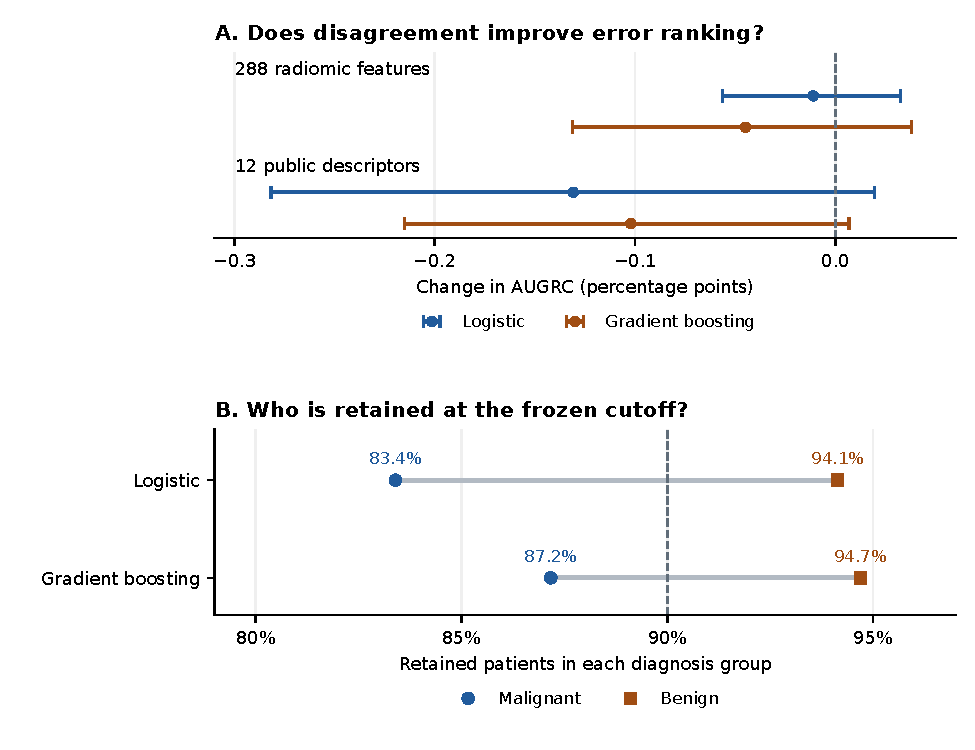
\includegraphics[width=\linewidth]{results.pdf}
\caption{A. Difference in fold-mean AUGRC for confidence plus disagreement versus confidence alone, with conditional paired 95\% intervals. Negative values favor the disagreement rule. B. Diagnosis-specific coverage for the confidence-only rule at cutoffs frozen on separate calibration patients. The dashed lines mark zero difference in A and the nominal coverage target in B.}
\label{fig:results}
\end{figure}

With confidence-only ranking at nominal 90\% coverage, logistic regression retained 219 of 265 malignant groups (82.6\%) and 512 of 546 benign groups (93.8\%). Gradient boosting retained 215 malignant groups (81.1\%) and 516 benign groups (94.5\%). Rounding within folds resulted in 90.1\% pooled coverage for both backbones.

\subsection{Frozen cutoffs and scanner transport}
The frozen confidence-only cutoff retained 735 of 811 patients (90.6\%) with logistic regression. It retained 221 of 265 malignant cases (83.4\%) and 514 of 546 benign cases (94.1\%). The coverage gap was 10.7 percentage points (conditional 95\% interval $[6.1,15.5]$). With gradient boosting the gap was 7.5 points ($[3.2,12.3]$), with 748 of 811 patients retained (92.2\%). Fold-level coverage ranged from 87.7\% to 95.1\% for logistic regression and from 90.2\% to 94.2\% for gradient boosting. Table~\ref{tab:frozen} gives the corresponding counts for the disagreement rules.

Every patient had a consistent device assignment. Three devices qualified for held-out testing, covering 800 paired patients. The fourth device (U-Systems) had 11 paired patients, of whom five were malignant. Across the three scanner holdouts, test coverage ranged from 92.5\% to 95.9\% and changes in AUGRC attributable to adding disagreement ranged from $-0.055$ to $+0.062$ points (Table~\ref{tab:devices}). The direction of the AUGRC change varied by device and backbone.

\subsection{Public-input sensitivity analysis}
With the 12 public descriptors, full-coverage accuracy was 84.8\% for logistic regression and 83.5\% for gradient boosting. The respective ROC areas were 0.908 and 0.888. The disagreement rule changed AUGRC by $-0.131$ points for logistic regression ($[-0.282,0.020]$) and $-0.102$ points for gradient boosting ($[-0.215,0.007]$). Both intervals include zero.

\section{Discussion}
The two backbones yielded small estimated changes in error ranking when we added absolute disagreement to confidence. The conditional intervals allow both improvement and worsening. The public-descriptor analysis yielded wider intervals. Mean margin and disagreement share a geometric constraint. A different representation, interaction, or disagreement measure could change the association. The analysis supports neither an equivalence claim nor a general conclusion that paired images have little value.

The frozen cutoff retained a smaller fraction of malignant cases for both backbones. A review queue built from this rule would therefore contain a disproportionate share of malignant cases in this cohort. Retained false negatives still occurred. The retrospective estimates describe queue composition and retained errors. Outcomes after human review and clinical utility require a separate evaluation.

The primary analysis uses two-image groups from one institution. The inputs rely on existing lesion masks and the results apply to the supplied images after lesion localization. The conditional bootstrap omits variation from refitting on overlapping training samples. Scanner holdouts test transfer within the same cohort. Differences may reflect case mix, acquisition procedure, or device. The study design cannot isolate those effects. The frozen threshold is an empirical cutoff without a nominal test-coverage guarantee. External testing requires an independent cohort with linked images, comparable descriptors, and reference diagnoses.

\section{Conclusion}
In 811 BUS-BRA patient groups with two images, we found uncertain incremental gains from adding absolute score disagreement to confidence. Diagnosis-specific retention revealed a difference that the overall coverage estimate would obscure, even when the cutoff was fixed using separate calibration patients.

\section{Data, reproducibility and disclosure}
The source collection and its publication describe acquisition and release conditions \cite{busbra,zenodo}. Exact replication of the radiomic analysis requires the frozen derived feature table. The public-input sensitivity analysis can be reproduced from the official archive and supplied code. The reproducibility package contains checksum-verifying runners, protocols, tests, and aggregate results. This secondary computational study used previously released anonymized data and collected no new data.

OpenAI Codex assisted implementation, testing, and manuscript drafting.

\clearpage
\appendix
\section{Operating points for the follow-up analyses}

\begin{table}[H]
\centering
\small
\caption{Frozen cutoff replay. Counts describe 811 paired test patients. Coverage is the percentage retained within each diagnosis. FN denotes retained malignant cases classified as benign.}
\label{tab:frozen}
\begin{tabular}{llrrrrr}
\toprule
Backbone & Rule & Retained & Malignant & Benign & Errors & FN\\
\midrule
Logistic & Confidence & 735 & 83.4\% & 94.1\% & 64 & 46\\
Logistic & With disagreement & 734 & 83.0\% & 94.1\% & 65 & 46\\
Boosting & Confidence & 748 & 87.2\% & 94.7\% & 70 & 53\\
Boosting & With disagreement & 747 & 86.4\% & 94.9\% & 69 & 50\\
\bottomrule
\end{tabular}
\end{table}

\begin{table}[H]
\centering
\small
\caption{Held-out scanner performance. The first number in each pair is for confidence alone and the second adds disagreement. AUGRC differences are in percentage points.}
\label{tab:devices}
\begin{tabular}{llrrrr}
\toprule
Test scanner & Backbone & Paired $n$ & Coverage (\%) & Retained errors & $\Delta$AUGRC\\
\midrule
GE Logiq 5 & Logistic & 319 & 93.1 / 95.9 & 31 / 34 & $-0.036$\\
GE Logiq 5 & Boosting & 319 & 95.3 / 94.0 & 23 / 22 & $+0.044$\\
GE Logiq 7 & Logistic & 414 & 93.2 / 92.5 & 68 / 68 & $+0.062$\\
GE Logiq 7 & Boosting & 414 & 94.0 / 94.4 & 46 / 46 & $-0.055$\\
Toshiba Aplio 300 & Logistic & 67 & 92.5 / 94.0 & 8 / 9 & $+0.045$\\
Toshiba Aplio 300 & Boosting & 67 & 92.5 / 95.5 & 10 / 11 & $+0.022$\\
\bottomrule
\end{tabular}
\end{table}

\begin{thebibliography}{9}
\bibitem{busbra}
W. G\'omez-Flores, M. J. Gregorio-Calas, and W. Coelho de Albuquerque Pereira.
BUS-BRA: A breast ultrasound dataset for assessing computer-aided diagnosis systems.
\emph{Medical Physics}, 51(4), 3110--3123, 2024.
\href{https://doi.org/10.1002/mp.16812}{doi:10.1002/mp.16812}.

\bibitem{zenodo}
W. G\'omez-Flores, M. J. Gregorio-Calas, and W. Coelho de Albuquerque Pereira.
BUS-BRA: A breast ultrasound dataset for assessing computer-aided diagnosis systems.
Zenodo, 2023. \href{https://doi.org/10.5281/zenodo.8231412}{doi:10.5281/zenodo.8231412}.

\bibitem{geifman}
Y. Geifman and R. El-Yaniv.
Selective classification for deep neural networks.
\emph{Advances in Neural Information Processing Systems}, 30, 2017.

\bibitem{wei}
T.-R. Wei, M. Hell, A. Vierra, R. Pang, Y. Kang, M. Patel, and Y. Yan.
Breast cancer detection on dual-view sonography via data-centric deep learning.
\emph{IEEE Open Journal of Engineering in Medicine and Biology}, 6, 100--106, 2025.
\href{https://doi.org/10.1109/OJEMB.2024.3454958}{doi:10.1109/OJEMB.2024.3454958}.

\bibitem{traub}
J. Traub, T. J. Bungert, C. T. L\"uth, M. Baumgartner, K. H. Maier-Hein,
L. Maier-Hein, and P. F. J\"ager.
Overcoming common flaws in the evaluation of selective classification systems.
\emph{Advances in Neural Information Processing Systems}, 37, 2024.
\href{https://doi.org/10.52202/079017-0076}{doi:10.52202/079017-0076}.

\bibitem{jones}
E. Jones, S. Sagawa, P. W. Koh, A. Kumar, and P. Liang.
Selective classification can magnify disparities across groups.
\emph{International Conference on Learning Representations}, 2021.
\href{https://arxiv.org/abs/2010.14134}{arXiv:2010.14134}.

\bibitem{kinalioglu}
I. H. Kinalioglu.
Device-specific conformal reliability under scanner-level acquisition shift in breast ultrasound CAD.
\emph{Medical Engineering \& Physics}, 2026.
\href{https://pubmed.ncbi.nlm.nih.gov/42833247/}{PMID:42833247}.

\bibitem{rutter}
C. M. Rutter.
Bootstrap estimation of diagnostic accuracy with patient-clustered data.
\emph{Academic Radiology}, 7(6), 413--419, 2000.
\href{https://doi.org/10.1016/S1076-6332(00)80381-5}{doi:10.1016/S1076-6332(00)80381-5}.
\end{thebibliography}
\end{document}
